    Наиболее простым видом столкновительно-индуцированных спектров являются трансляционные спектры, порождаемые смесью двух благородных газов при низком давлении, где доминируют бинарные столкновения. При более высоких давлениях будут случаться столкновения с участием трех и более атомов, которые будут видоизменять форму спектра поглощения. На рис. \ref{pic-two-atom-experiment} приведены примеры экспериментальных столкновительно-индуцированных спектров поглощения в дальней ИК области систем He$-$Ar, Ne$-$Ar и Ar$-$Kr \cite{frommhold}. Было экспериментально подтверждено, что интенсивность поглощения линейно зависит от произведения плотностей газов $\rho_1 \rho_2$, что говорит о том, что спектр порождается парами разных атомов. Отклонение от линейной зависимости будет говорить о том, что при данных концентрациях существенный вклад вносят многочастичные столкновения. Спектры, изображенные на рис \ref{pic-two-atom-experiment}, сняты при разных концентрациях от 60 амага (He$-$Ar) до 200 амага (Ar$-$Kr).  

\begin{figure}[H]
    \centering
    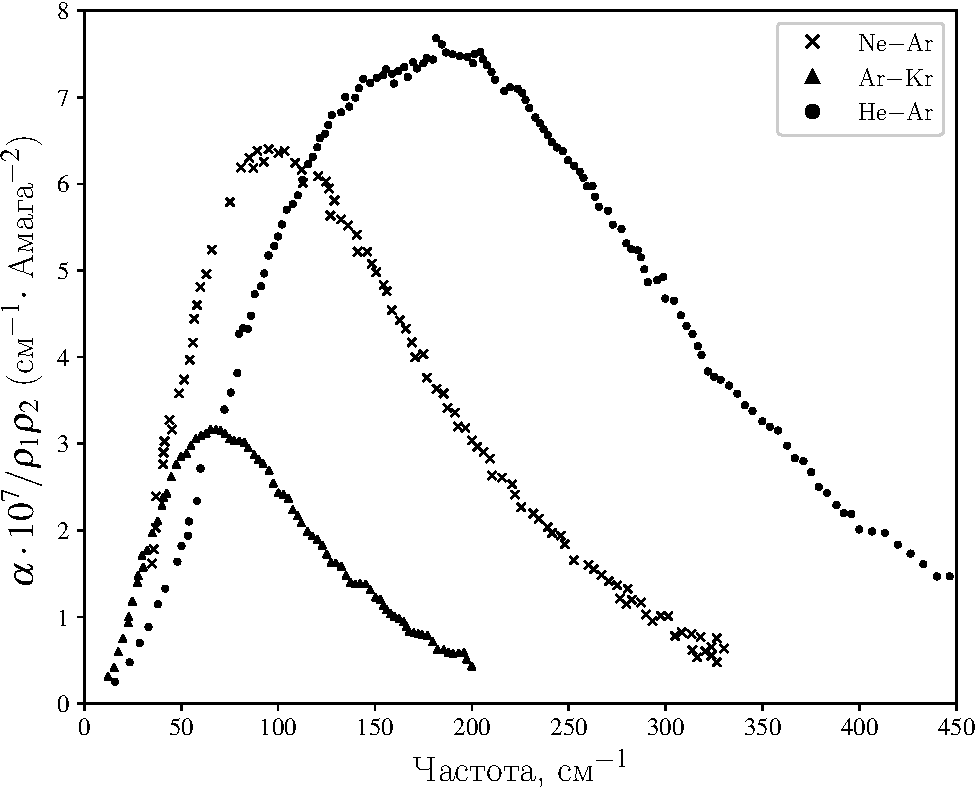
\includegraphics[width=0.7\linewidth]{./pictures/twoatom_experiment/experiment_diatom_spectra-crop.pdf}
    \label{pic-two-atom-experiment}
    \caption{Экспеиментальные спектры бинарного поглощения систем гелий$-$аргон, неон$-$аргон и аргон$-$криптон при комнатной температуре \cite{frommhold}}
\end{figure}

В работе \cite{kranendonk1973} авторы разрабатывают формализм расчета столкновительно-индуцированного спектра в приближении бинарных столкновений. Авторы рассматривают систему, состояющую из молекулы $H_2$, возмущенной атомами $Ar$. Вращательное движение молекулы $H_2$ исключено из рассмотрения -- обе сталкивающихся молекулы рассматриваются как безструктурные сферически-симметричные частицы. \par
    Спектральная функция, определяющая профиль спектра поглощения, связана с функцией автокорреляции суммарного дипольного момента системы преобразованием Фурье
\begin{gather}
    J(\omega) = \intty \mean{ \bs{\mu}(0) \bs{\mu}(t) } e^{i \omega t} dt .
\end{gather} 
В приближении бинарных столкновений корреляционная функция суммарного дипольного момента становится 
\begin{gather}
    \mean{ \bs{\mu}(0) \bs{\mu}(t) } = N \mean{ \bs{\mu}_1(0) \bs{\mu}_1(t) },
\end{gather} 
%
где через $\bs{\mu_1}(t)$ обозначен дипольный момент индуцированный квадрупольным полем молекулы $H_2$ на атоме $Ar$, а $N$ -- количество рассматриваемых пар. Приведенную массу системы обозначают через $\mu$; вектор, соединяющий центр масс молекулы $H_2$ атомом $Ar$ -- через $\mathbf{R}$; потенциал взаимодействия -- через $V(R)$ $[$как уже говорилось, вращательное движение молекулы водорода не рассматривается, поэтому потенциал зависит только от расстояния между центрами масс $R$$]$. \color{red}{Затем как-то получают следующее выражение для корреляционной функции}
\color{black}{}
\begin{gather}
    C(t) = \frac{N}{V} \lb \frac{\mu}{2 \pi k T} \rb^{3/2} \iint \bs{\mu}_1(\mathbf{R}) \cdot \bs{\mu}_1(\mathbf{R}(t)) \exp \lb -\frac{\mu \dot{\mf{R}}^2}{2 k T} +  \frac{V(R)}{k T} \rb d \mathbf{R} d \dot{\mathbf{R}},
\end{gather}
%
где $\mathbf{R}(t)$ -- значение $\mathbf{R}$, вычисленное в момент времени $t$, вычисляется путем расчета классической траектории, начальными условиями для которой взяты $\mf{R}$ и $\dot{\mf{R}}$.


